\chapter{\label{chap:konzeption}Konzeption}
Die erarbeiteten Anforderungen zur Untersuchung der Konfliktmanagementstrategien offlinefähiger Systeme werden in diesem Kapitel für die Konzeption angewendet.\\
Es soll für jede zu untersuchende Technologie ein Prototyp entwickelt werden. Im Rahmen dieser Arbeit entsteht ein Prototyp der \sc{Redux Offline} verwendet und ein zweiter in dem PouchDB und CouchDB eingesetzt wird. Für letzteren könnte genausogut das Framework \sc{Hoodie} benutzt werden, da es sowohl PouchDB als auch CouchDB benutzt~\cite{hoodie-how}. Doch da für den zu entwickelnden Prototyp lediglich diese beiden Komponenten benötigt werden, wurde sich dagegen entschieden.
Bis zu einem gewissen Status, nämlich dem der Verwendung der Technologien, sind beide Prototypen -- bis auf den Namen-- identisch.
% Beginnend mit dem Aufbau der exemplarischen Anwendung werden in den folgenden Abschnitten die  der Anwendungsaufbau, Architektur  und schließlich \todo{blabla} die graphische Oberfläche aufgeführt.
% Den Raum aller möglichen Lösungen anhand der Anforderungen auf die in irgendeinem Sinn beste / geeignetste einzuschränken:\\
% App entwickeln, in der es einen `Verbindung unterbrechen` Knopf gibt ', oder ob es aus irgendwelchen Erwägungen notwendig sein könnte, das über eine separate Instanz zu machen.
%
% Aufbau
%
\section{Anwendungsaufbau}
Die Prototypen bestehen im Frontend aus React und wurden mit \sc{Create React App} erstellt. \sc{Create React App} erstellt ein Projekt mit dem gewünschten Namen, generiert eine initiale Projektstruktur (vgl. Abbildung \ref{fig:init}) und installiert die dafür benötigten Abhängigkeiten~cite{create-react}. Diese sind im Verzeichnis node\_modules installiert.
Außerdem ist ein ServiceWorker und ein App Manifest (\tt{manifest.json}) enthalten, wodurch die \gls{PWA}-- Kriterien erfüllt sind.\\
Als Template gibt es nun die \tt{public/index.html}-- Datei. In der \tt{index.js}--Datei werden die React--Komponenten und der ServiceWorker initialisiert.. Alle \tt{App.*}--Dateien umfassen eine minimale Beispielanwendung.
In der generierten \tt{package.json}--Datei (vgl. Abbildung \ref{fig:init2}), befinden sich Informationen über die Anwendung und ihre Abhängigkeiten. Im Unterpunkt \tt{scripts} werden Kommandozeilen-Aufrufe definiert und können mit dem Befehl \tt{npm} aufgerufen werden.
\begin{figure}[h]
  \centering
  \begin{subfigure}[t]{0.45\textwidth}
          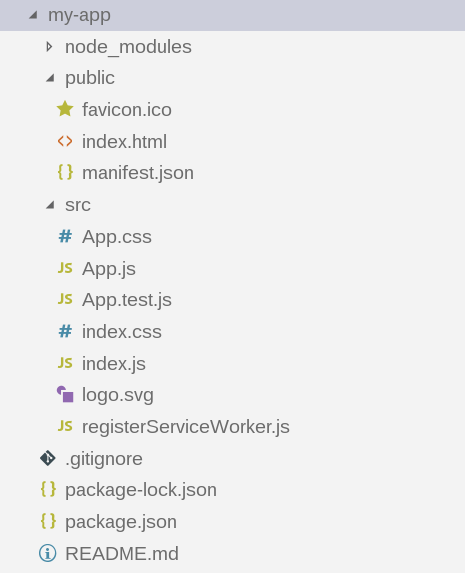
\includegraphics[width=\textwidth]{Ordnerstruktur}
          \caption{Die initiale Projektstruktur}
          \label{fig:init}
  \end{subfigure}
  ~ 
  \begin{subfigure}[t]{0.45\textwidth}
          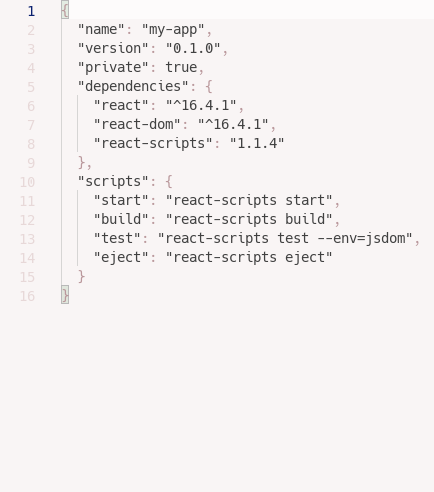
\includegraphics[width=\textwidth]{rca-package}
          \caption{Die initiale package.json Datei}
          \label{fig:init2}
  \end{subfigure}
  \grayRule
  \caption[Create React App: initiale Testapplikation]{einer mit Create React App erstellten Testapplikation}
  \label{fig:create-react-app}
\end{figure}
%
% React Komponenten
%
\sub{Aufbau der React Komponenten ?}
React ist eine open-source Bibliothek, die dazu dient, die View-Komponente des Model-View-Controller-Ansatzes abzudecken, also die Seite der Anwendung die für die Anzeige und Interaktion zuständig ist. Ein Vorteil von React sind die wiederverwendbaren Komponenten. Eine Komponente ermöglicht die Aufteilung der UI in kleine Teile und ist eine abstrakte Basisklasse. Einmal implementiert, lässt sich eine Komponente immer wieder verwenden~\cite{react}.\\

Zur Veranschaulichung beschreibe ich anhand des Listings \ref{code:react-list} die Komponente der Kontaktliste, so wie sie im Startbildschirm angezeigt wird.
\begin{center}
\lstinputlisting[language=REACT,caption={React Komponente \tt{ContactList} der Prototypen}, label=code:react-list]{code/List.js}
\end{center}
%
% Redux
%
\subsub{Redux}
%
%
% Architektur
%
\section{Architektur}
Die zu erstellenden Prototypen erhalten die Namen \it{amilia-qouch} und \it{amilia-rdx}, wobei Amilia der Name ist, der sich in den Beispielkontakten in den Szenarien wiederfindet. Die Abkürzung \it{rdx} steht für Redux und zeigt, dass dieser Prototyp \sc{Redux Offline} verwendet. Die Endung \tt{qouch} soll die Symbiose von CouchDB und PouchDB darstellen. Der Buchstabe Q klingt wie das hart ausgesprochene C in Couch und wenn man das kleine Q horizontal spiegelt, sieht man das P für Pouch.\\\\
Beide Prototypen setzen sich aus den nachfolgend beschriebenen Komponenten zusammen, welche in Abbildung \ref{fig:uml} veranschaulicht werden.\\\\
Die Komponente \tt{Contacts} fungiert als Container und ist das Herzstück der Anwendung. Er definiert die graphische Oberfläche und stellt alle notwendigen Funktionen bereit. Sie hat einen internen \tt{state} in dem sowohl die Kontaktliste, als auch die Daten für das Formular gespeichert sind. Im Diagramm ist der \tt{state} an der blauen Schrift zu erkennen. Das Objekt \tt{editView} zeigt, welche Ansicht -- Liste oder Formular -- gerade aktuell ist und speichert den im Formular zu ladenden Kontakt. Wie das Kontaktobjekt aufgebaut ist zeigt der blaue Kasten im Diagramm. Wird eine Aktion zum Ändern der Ansicht aufgerufen, beispielsweise durch das Betätigen eines Knopfes, wird über die Funktion \tt{toggleEdit()} der interne \tt{state} aktualisiert und ein erneutes Rendern der Komponente eingeleitet. Dann wird entsprechend die Liste oder das Formular gerendert.\\
Die \tt{Header}--Komponente zeigt den Netzwerkstatus der Anwendung an und hat einen Knopf, der zum \tt{ContactForm} führt.\\
Die \tt{ContactList} wird initial gerendert. Es werden alle Kontakte als Liste dargestellt. Hier kann das Bearbeiten (\tt{handle"-On"-Edit"-Click()}) oder das Löschen (\tt{handle"-On"-De"-lete"-Click()}) des Kontakts eingeleitet werden.
\begin{figure}[H]
  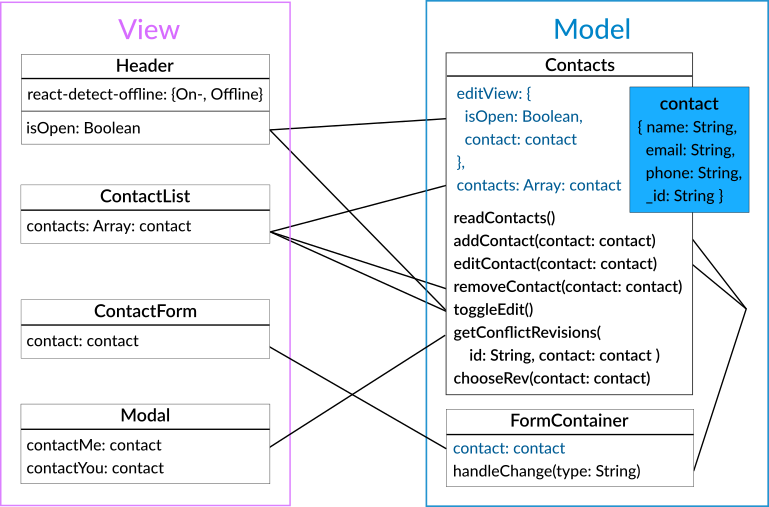
\includegraphics[width=\textwidth]{uml}
  \grayRule
  \caption{Komponentenarchitektur}
  \label{fig:uml}
\end{figure}
Die Komponente \tt{ContactForm} zeigt, sofern vorhanden, alle im Kontakt gespeicherten Daten an. Diese können hier bearbeitet werden. Gibt es keine Kontaktdaten die geladen werden kann, kann hier ein neuer Kontakt angelegt werden. Zusätzlich zu den Eingabefeldern für jedes Kontaktattribut hat sie zwei Knöpfe mit denen die Aktion bestätigt (\tt{handleSubmit()}) oder abgebrochen (\tt{handleCancel()}) werden kann. Sie ist neben \tt{Contacs} die einzige Komponente mit einem internen \tt{state}. Dieser wird für die Ereignishandler benötigt, die auf die Veränderung der einzelnen Eingabefelder zu ``lauschen``. Der zu bearbeitende Kontakt wird hier zwischengespeichert und dann als Ganzes an \tt{Contacts} gegeben.\\
\todo{Konflikt--Dialog}\\\\
%
% 
%
\todo{Backend: Implementierung bei qouch nicht notwendig. Nur Installation von Couch.\\ 
Für Redux Offline: Server und JSON Datei als DB Ersatz?}
% Client - Server - Modell
\begin{figure}[H]
  \centering
  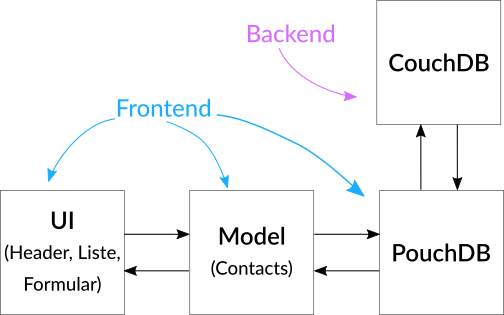
\includegraphics[width=0.8\textwidth]{qouch-model}
  \grayRule
  \caption{Client-Server-Modell}
  \label{fig:qouch-model}
\end{figure}
%
% Lokale Speicherung
%
\sub{Lokale Speichern der Daten}
Das Seichern von Kontakten ...
Beide Technologien benutzen unterschiedliche ... 
PouchDB nimmt IndexedDB oder... Browserabhängig.\\
Redux Offline nimmt per default localStorage, das kann aber konfiguriert werden.
% Redux Offline
\subsub{Lokale Speicherung mit Redux Offline}
Redux Offline: Idee: Store = Datenbank
% Pouch
\subsub{Lokale Speicherung mit PouchDB}
%
% Sync
%
\sub{Synchronisation}
% Redux Offline
\subsub{Synchronisation mit Redux Offline}
Redux Offline: Server der alle \gls{CRUD} Operationen unterstützt,
\gls{JSON}--Datei zur Persisierung um Ergebnisse nicht zu verfälschen 
Redux Offline: Idee: Store = Datenbank
% Pouch
\subsub{Synchronisation mit PouchDB}
CouchDB = RemoteDB\\
% -----------------------------------------------------------------------------
%
% Online / Offline
%
\sub{Verbindungsstatus feststellen und ändern}
Für die Überprüfung der Verbindung zum Server wird das Modus \sc{React Detect Offline} verwendet. Es beobachtet den Online-- und Offlinestatus und bietet zwei Komponenten entsprechend des Status den Inhalt rendern. Der folgende Codeausschnitt zeigt eine Verwendung dieser beiden Komponenten. Ist die Anwendung online, wird `you are online` gerendert. Im anderen Fall ~`you are offline`.
%
\begin{center}
\lstinputlisting[language=REACT,caption={Beispiel einer React Detect Offline Implementierung}, label=code:react-detect]{code/Header.js}
\end{center}
%
Das Modul fragt alle fünf Sekunden die URL \url{https://ipv4.icanhazip.com} ab und rendert je nach Verbindungsstatus die entsprechende Komponente. Verschiedene Parameter wie die URL oder das Poll--Interval können konfiguriert werden~\cite{react-detect}.\\\\
%
Der Verbindungsstatus kann im Browser geändert werden. Die Prototypen, die im Rahmen dieser Arbeit entwickelt werden, sollen in den Browsern Firefox und Chromium laufen.\\
In Firefox lässt sich der Netzwerkstatus über das Einstellungsmenü ändern. Dort kann man entweder unter dem Punkt `Sonstiges` oder dem Punkt `Web-Entwickler` `Offline arbeiten` auswählen und ist vom Internet getrennt. Dieser Status lässt sich über den selben Weg rückgängig machen.\\
In Chrome öffnet man dazu die Entwicklertools, geht auf `Netzwerk` und klickt auf die Checkbox `Offline` am oberen Rand. Dieselbe Checkbos ist auch im `Application`--Tab unter `Service Workers` zu finden.
%
% UI
%
\section{Die graphische Oberfläche}
Aus den minimalen Anforderungen an die graphische Oberfläche ergibt sich das Design. Anhand der folgenden Abbildungen werden die gefertigten Entwürfe der BenutzerInnenoberfläche dargestellt.\\\\
Diese Listenansicht in Abbildung \ref{fig:list} besteht aus dem Header / Kopf und den Listeneinträgen. Sie zeigt die Kontakteinträge in beiden Netzwerkstatus: online (Abbildung \ref{fig:list-online}) und offline (\ref{fig:list-offline}).\\\\
Im Header ist abzulesen ob die Anwendung gerade eine Netzwerkverbindung hat oder nicht. Für eine bessere Prägnanz wurden hierzu unterstützend die Farben Rot für keine Verbindung und Grün für eine bestehende Netzwerkverbindung gewählt. Rechts im Header gibt es einen Knopf mit dem man in die Ansicht gelangt in der ein Kontakt hinzugefügt werden kann.\\
In der Liste sieht man die Namen der Person und jeweils einen Knopf zum Bearbeiten oder Löschen. Mit der Betätigung des `Delete`--Knopfs wird der entsprechende Eintrag in der Liste gelöscht
\begin{figure}[H]
  \centering
  \begin{subfigure}[t]{0.49\textwidth}
          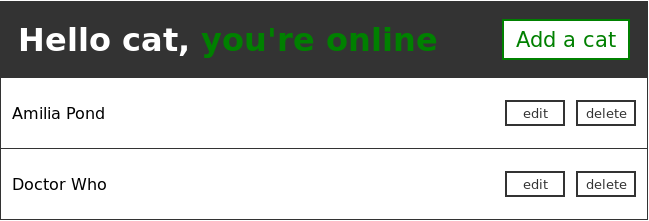
\includegraphics[width=\textwidth]{list-online}
          \caption{Kontaktliste im Onlinestatus}
          \label{fig:list-online}
  \end{subfigure}
  ~ 
  \begin{subfigure}[t]{0.49\textwidth}
          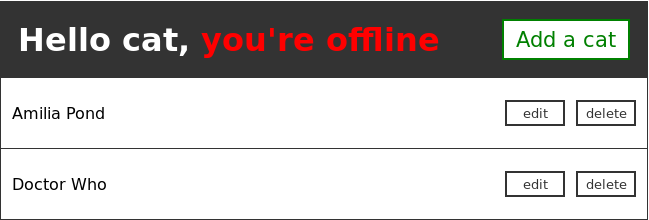
\includegraphics[width=\textwidth]{list-offline}
          \caption{Kontaktliste im Offlinestatus}
          \label{fig:list-offline}
  \end{subfigure}
  \grayRule
  \caption{Die Kontaktliste in beiden Netzwerkstatus}
  \label{fig:list}
\end{figure}
Klickt man auf den Knopf zum Bearbeiten oder auf den zum Hinzufügen eines Kontakts gelangt man in die Bearbeitungsansicht (vgl. Abbildung \ref{fig:edit}). Der Header ist bis auf den Knopf zum Hinzufügen eines Kontakts identisch zu dem der Liste. Auch hier ist abzulesen ob die Anwendung on-- oder offline ist. Da man sich bereits in der Ansicht zum Anlegen oder Editieren eines Kontaks befindet, ist der Knopf im Header überflüssig.\\
Ein Kontakt hat einen Namen, eine E-Mailadresse und eine Telefonnummer. In dieser Ansicht gibt es für jedes Attribut ein Eingabefeld. Die Felder sind beim Bearbeiten des Kontakts vorausgefüllt. Mittels Betätigung des `Speichern` Knopfs werden die Änderungen übernommen, klickt man auf `Cancel` werden sie verworfen. In beiden Fällen gelangt man wieder zur Listenansicht.
\begin{figure}[H]
  \centering
  \begin{subfigure}[t]{0.49\textwidth}
          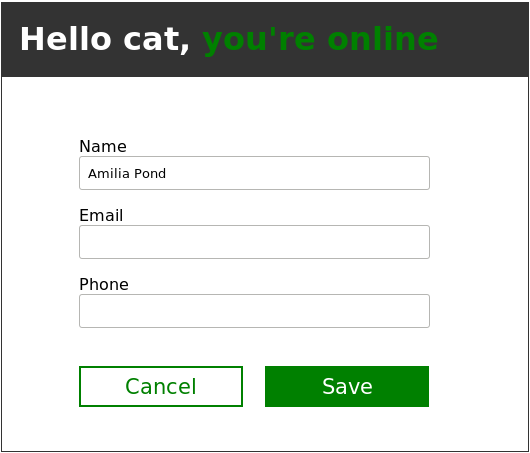
\includegraphics[width=\textwidth]{edit}
          \caption{Editieransicht im Onlinestatus}
          \label{fig:edit-online}
  \end{subfigure}
  ~ 
  \begin{subfigure}[t]{0.49\textwidth}
          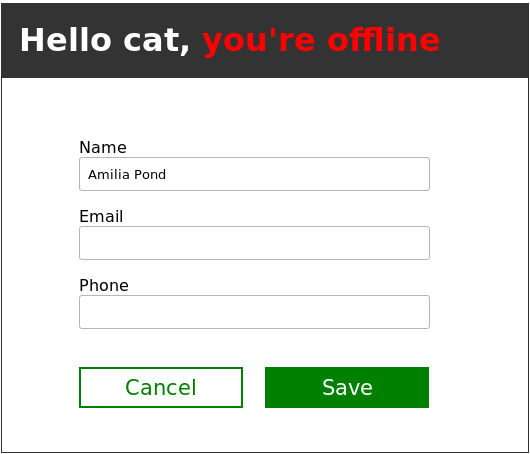
\includegraphics[width=\textwidth]{edit-offline}
          \caption{Editieransicht im Offlinestatus}
          \label{fig:edit-offline}
  \end{subfigure}
  \grayRule
  \caption{Die Editieransicht in beiden Netzwerkstatus}
  \label{fig:edit}
\end{figure}
\todo{Konfliktdialog}
%
% Testfälle
%
\section{Testfälle}
Folgende Testfälle werden während der Entwicklung stetig durchgeführt. Das erfolgreiche Bestehen dieser Tests ist eine notwendige Qualitätseigenschaft der zu entwickelnden Prototypen.
\begin{description}[leftmargin=0.7cm,style=nextline]
\item[Netzwerkstatus:] 
Die Anwendung muss zu jeder Zeit den korrekten Netzwerkstatus anzeigen.\\
\item[Kontakte lesen:] 
Die Anwendung bei jedem Start die Kontakte aus dem lokalen Speicher oder aus der \it{Datenbank} laden.\\
\item[Kontakt anlegen:] 
Die Anwendung muss zu jedem Zeitpunkt in der Lage sein einen Kontakt mit jedem seiner Attribute anzulegen. Dazu muss er immer lokal gespeichert werden und sobald eine Internetverbindung besteht, persistiert werden.
Das Anlegen eines Kontakts im Offlinestatus ist für die Konfliktforcierung erforderlich.\\
\item[Kontakt bearbeiten:] 
Die Anwendung muss zu jedem Zeitpunkt in der Lage sein einen Kontakt mit jedem seiner Attribute zu bearbeiten. Ist keine Internetverbindung vorhanden, müssen die Änderungen lokal übernommen und später, sobald sich der Netzwerkstatus ändert, synchronisiert werden.
Das Bearbeiten eines Kontakts im Offlinestatus ist für die Konfliktforcierung erforderlich.\\
\item[Kontakt löschen:] 
Die Anwendung muss zu jedem Zeitpunkt in der Lage sein einen Kontakt zu löschen.
Das Löschen eines Kontakts im Offlinestatus ist für die Konfliktforcierung erforderlich.
\end{description}